\begin{frame}
    \centering
    \begin{figure}[H]
        
\includegraphics[keepaspectratio, width=0.7\paperwidth, height=\paperheight]{LeeLogo}
    \end{figure}
    Informatik: Data Science und Sicherheit\\
    \textbf{Zahlensysteme} \emoji{pencil}: \textbf{Lektion 01}
\end{frame}

\begin{frame}{Historischer Hintergrund}{Was ist Informatik?}
\begin{center}
``\textit{Informatik}'' = ``Information'' + ``Automatik''
\end{center}
Wissenschaft der \textbf{automatischen}...
\begin{itemize}
\item Darstellung...
\item Speicherung...
\item Übertragung...
\item Verarbeitung...
\end{itemize}
...von Informationen / \textbf{Daten}.
\end{frame}

\begin{frame}[fragile]{Was sind \textit{Daten}?}
  \textbf{``Daten''} = Plural von \textit{Datum}
  \begin{itemize}[<+->]
    \item \textit{Datum} = Fakt(um) (von lateinisch \textit{datum} = gegeben, \textit{dare} = geben), also etwas \textbf{Gegebenes}\\
          Beispiel:
          \begin{itemize}
            \item ``Mein Nachbar heisst Marco Odermatt.''
            \item ``Aktuell findet an der KLW Unterricht statt.''
            \item ``Das Billett von Zürich nach Winterthur kostet CHF 6.80.''
            \item ``Das Logo der KLW besteht aus blauen und roten Farben.''
            \item ...
          \end{itemize}
    \item In der \textbf{Informatik}: irgendetwas mit Nullen und Einsen\\
          Beispiel:
          \begin{itemize}
            \item \ldots\verb|10100010101111011101001001|\ldots
            \item \ldots\verb|11101110110000111011010111|\ldots
            \item \ldots
          \end{itemize}
    \item Welche Codierung welchem \textit{Datum} entspricht, bestimmt der / die ProgrammiererIn
  \end{itemize}
\end{frame}

\begin{frame}{}
\begin{center}
Was ist überhaupt eine Zahl? Woher stammen Zahlen?
\end{center}
\end{frame}

\begin{frame}{Historischer Hintergrund}{Ishango-Knochen}
	\begin{columns}
	\begin{column}{0.5\textwidth}
		\begin{figure}[H]
			\centering
			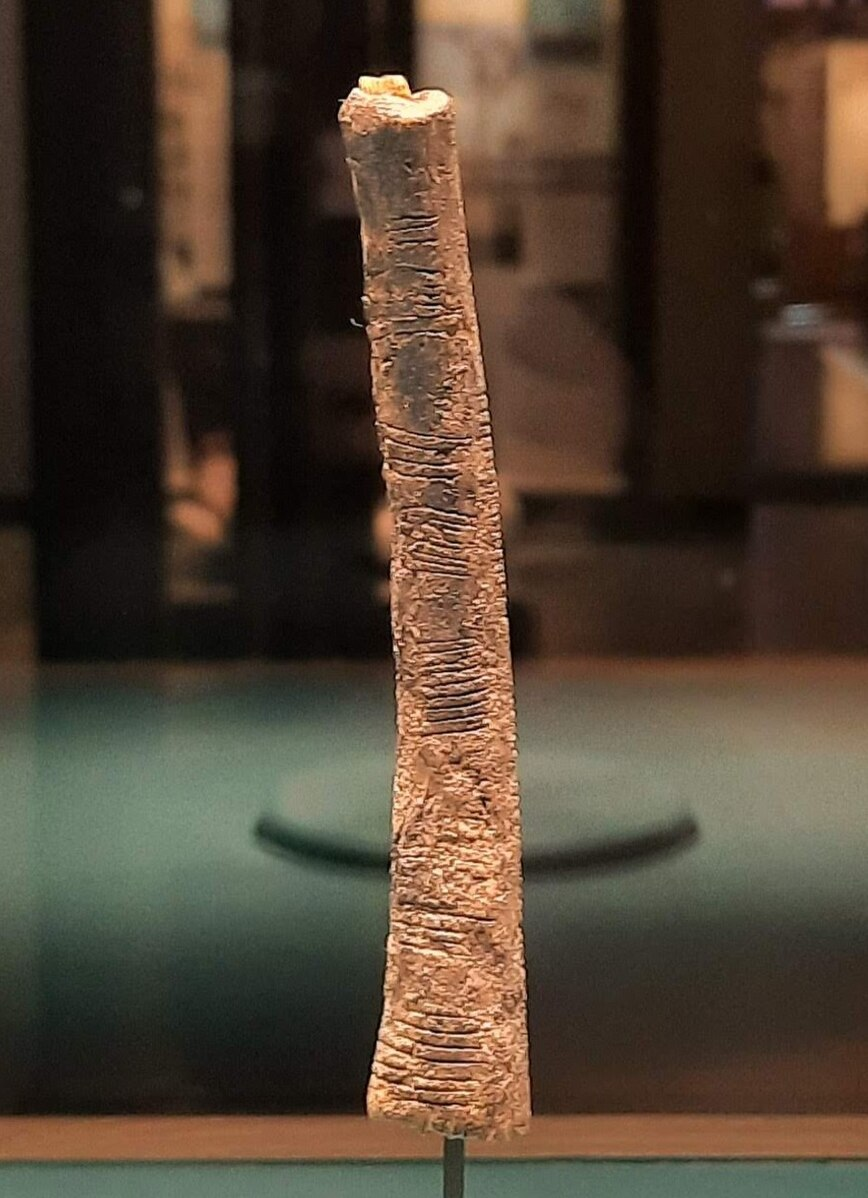
\includegraphics[height=.7\pageheight]{GrundlagenInfo/DataScience/01_TheoretischeInformatik/Figures/ishango-bone}
			\end{figure}
		\end{column}
		\begin{column}{0.5\textwidth}
			\begin{itemize}
			\item \emoji{apple}\emoji{apple}\emoji{apple} = ?
			\item \emoji{fish}\emoji{fish}\emoji{fish} = ?
			\end{itemize}
		\end{column}
	\end{columns}
\end{frame}

\begin{frame}{Historischer Hintergrund}{\textit{Unäre} Zahlendarstellung}
\begin{equation*}
	\text{drei Kerben} \quad\leftrightarrow\quad \twemoji{tropical fish}\twemoji{tropical fish}\twemoji{tropical fish} \quad\leftrightarrow\quad |||
	\quad\leftrightarrow\quad \text{\textbullet\textbullet\textbullet}
\end{equation*}
\begin{center}
Was könnten Nachteile dieser Zahlendarstellung sein?
\end{center}
\only<2->{
\begin{center}
||||||||||||||||||||||||||||||||||||||
\end{center}
\begin{itemize}
\item Wie liest man diese Zahl?
\item Speicherbedarf!
\end{itemize}
}
\end{frame}

\begin{frame}{Zahlensysteme mit Basisgrössen}{Römische Zahlen}

\begin{center}
Basisgrössen: $I$ (Eins), $V$ (Fünf), $X$ (Zehn), $L$ (Fünfzig), $C$ (Hundert), $D$ (Fünfhundert) und $M$ (Tausend).
\end{center}
\begin{center}
Welche Zahl ist das?
\end{center}

  \begin{equation*}
    CCCCCLIIII
  \end{equation*}
  
\only<2->{\begin{center}
545 $\rightarrow$ Gibt es Vereinfachungsmöglichkeiten?
\end{center}}
\only<3->{

  \begin{equation*}
    DLIV
  \end{equation*}
  }

\only<4->{\emoji{coin} Basisgrössen können wie \textbf{Münzen} angeschaut werden \emoji{coin}}
\end{frame}

\begin{frame}{Zahlensysteme mit Basisgrössen}{Münzendarstellung}
Eine Sammlung von Münzen nennen wir die Münzendarstellung einer Zahl \textit{m}, wenn
\begin{itemize}
\item \textbf{Korrektheit}: die Zahl \textit{m} gleich der Summe der Münzenwerte ist.
\item \textbf{Minimalität}: keine Sammlung mit weniger Münzen existiert, deren Summe \textit{m} ist.
\end{itemize}

Beispiel: LXXV ist die alte römische Münzendarstellung von 75

\end{frame}


\begin{frame}{Zahlensysteme mit Basisgrössen}{Münzendarstellung}

Wir haben folgende Münzen: \coin{1}\coin{2}\coin{3}\coin{5}\coin{10}\\

Wie stellt man die Zahl 4 dar?

\only<2->{
\begin{itemize}
\item \coin{1}\coin{3}
\item \coin{2}\coin{2}
\end{itemize}}
\only<3->{
$\rightarrow$ Problem: Münzdarstellung ist zwar \textit{minimal}, aber nicht \textit{eindeutig}
}
\end{frame}

\begin{frame}{Wichtige Beobachtung zu Ziffern}
\begin{itemize}[<+->]
\item Beispiel: Wir wollen 13 Objekte im Dezimalsystem mit so wenigen \enquote{Münzen} (Potenzen der 10) wie möglich darstellen. Wir könnten dies mit 13 Einern tun. Doch wir sehen sofort, dass sich 10 Einer stets durch nur einen einzigen Zehner (und null Einer) ersetzen lassen. Dadurch haben wir 9 Münzen gespart.
\begin{itemize}
    \item Verfügbare Münzen: \coin{1}, \coin{10} etc.
    \item Münzen vorher:\\
    \coin{1}\coin{1}\coin{1}\coin{1}\coin{1}\\
    \coin{1}\coin{1}\coin{1}\coin{1}\coin{1}\\
    \coin{1}\coin{1}\coin{1}\\
    \item Münzen nachher:\\
    \coin{10}\coin{1}\coin{1}\coin{1}\\
\end{itemize}
\item In einem $b$-adischen System haben wir also maximal $b-1$ viele Münzen vom Typen $b^k$, denn sonst würden wir stets Gruppen von je $b$ vielen Münzen vom Typ $b^k$ durch eine einzige Münze vom Typen $b^{k+1}$ ersetzen und hätten dadurch, für jede solche Gruppe, $b-1$ Münzen eingespart.
\end{itemize}

\end{frame}


\begin{frame}{Wichtige Beobachtung zu Ziffern}
Angenommen wir haben in einem Münzsystem (nicht zwingend einem $b$-adischen) eine Münze, die genau $k$-mal ($k>1$ ist eine natürliche Zahl) so gross ist wie die nächst kleinere Münze. Dann werden wir höchstens $k-1$ viele der kleineren Münzen verwenden. Ansonsten würden wir nämlich stets Gruppen von $k$ der kleineren Münzen durch eine der grösseren ersetzten und erhielten, für jede solche Gruppe, eine um $(k-1)$ Münzen kürzere Darstellung.
\begin{itemize}
    \item Beispiel:\\
    Verfügbare Münzen: \coin{5}, \coin{15}, \coin{45} etc. (Vergrösserungs-Schritt 3)\\
    \coin{5}\coin{5}\coin{5} $\rightarrow$ \coin{15} (Reduktion um 2 Münzen)\\
    \coin{15}\coin{15}\coin{15} $\rightarrow$ \coin{45} (Reduktion um 2 Münzen)
\end{itemize}
\end{frame}

\begin{frame}{Fazit}
    \begin{itemize}
    \item Zahlensysteme sind ``willkürlich'' und historisch entstanden
    \item Erste Zahlensysteme funktionierten als Münzendarstellungen
        \item Computer arbeiten mit binären Zahlen \{0,1\}
        \begin{itemize}
            \item Schnelleres Rechnen
            \item \emoji{high-voltage} 1 = Strom fliesst, 0 = kein Strom
        \end{itemize}
    \end{itemize}
\end{frame}

\begin{frame}{Aufgaben}{Skript ``Theoretische Informatik'' (auf Moodle)}
\aufgabebox{Aufgabe 1.1}
\end{frame}